
\chapter{Introduction} % Main chapter title

\label{Chapter 1} % For referencing the chapter elsewhere, use \ref{Chapter1} 

\lhead{Chapter 1 . \emph{Introduction}} % This is for the header on each page - perhaps a shortened title


Researchers in Artificial intelligence, and especially in the field of automated reasoning and problem resolving, are interested on the representation of the real world using logical models to define processing algorithms for these models. The reasoning about actions and changes is one of the fields in the IA which is particularly interested to some problems involving world changes. In particularly, since the 80s, Planning allowed to propose several automatic methods that, from an initial state, a goal state and a set of actions described as transitions between states, build a sequence of actions that lead from the initial state to the goal state.
\par Once the plan is built, it will be executed by the controller of the physical system. However, sometimes during the execution, the current state may not correspond to the expected state. Therefore, the controller can no more proceed with the plan. This is called a breakdown.

These breakdowns can be caused by dynamic environment (extern actions that modify the system states), or by an incomplete modeling of the real system. The planner needs, in order to build a consistent plan, a complete and a faithful representation of the problem actions: knowledge domain. 
Nevertheless, modeling such complete domain will require significant knowledge-engineering effort if it is not impossible \cite{gil1992acquiring}. For example, if we want to represent the human activity in housing for the intelligent management of energy \cite{hurauxmodele}, such as cooking dishes task. The most challenging part in  modeling this task is to define the level of granularity with which we can construct a model that represent  accurately  the real world which implies representing each  action of cooking and devices taking into account the variability of the environment. constructing such model is so time consuming even impossible. Thus, the existing models represent the general view of the world as showed in the figure \ref{Cooking model example} that represent the cooking example.

   In the real life, we frequently observe a combination of these two phenomena: an incomplete model and a dynamic environment. Therefore, it is necessary to define plan repair in order to face possible breakdowns. This represents the topic of my master thesis that we will present here.
\par The goal of our approach is to build a system that can recover from breakdowns taking into account the incompleteness of the model. Unlike the existing systems which suppose that the model is pretty complete to be consistently fixed and the breakdowns are only caused by the dynamic nature of the environment. 
\par In the following, we will present the existing works in this domain. The chapter 2 presents the linear methods of planning, the hierarchical planning and the reactive approaches and discussing their advantages and limits. In the chapter 3, I propose a hybrid model that combines the execution of a reactive HTN with classic planning models of plan reparation. In the fourth section, I present the proposed implementation of this model, the experiments and validation of the proposed solution . We conclude this thesis by the future works. 
\begin{figure}[h]
	\centering
	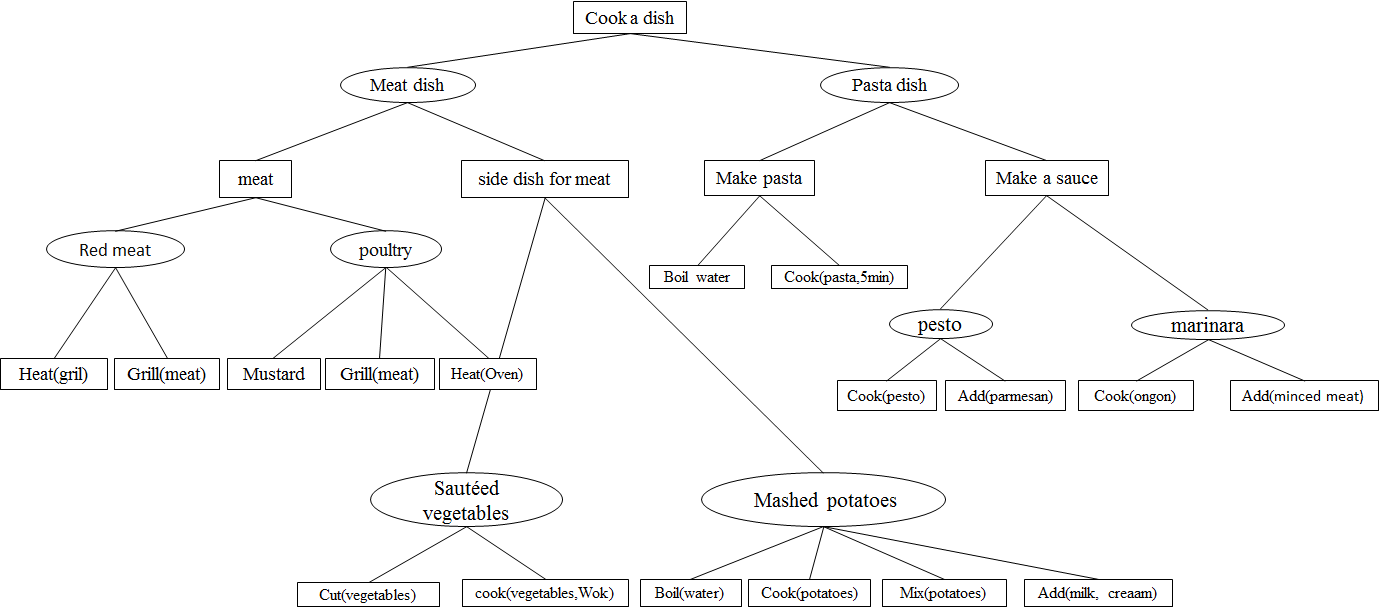
\includegraphics[width=\columnwidth]{Pictures/cooking.png}
	\caption{\label{Cooking model example} Cooking model example}
\end{figure}
